En aquest capítol explicarem el disseny del projecte. 
S'ha dividit en dues parts per facilitar l'organització. 
La primera part explica la interfície, el sistema d'estats del motor, i l'editor de prefabs. 
La segona explica l'estat del joc on el jugador té control del personatge, també anomenat \textit{gameplay}. 
Hi ha una secció addicional per explicar el funcionament de les llibreries utilitzades, així com altres eines petites que poden ser difícils d'ubicar en cap de les dues parts principals.
A la figura~\ref{dc_general} es mostren la majoria de classes del projecte, i les principals relacions entre elles.
\pagebreak
\begin{figure}[H]
  \centering
  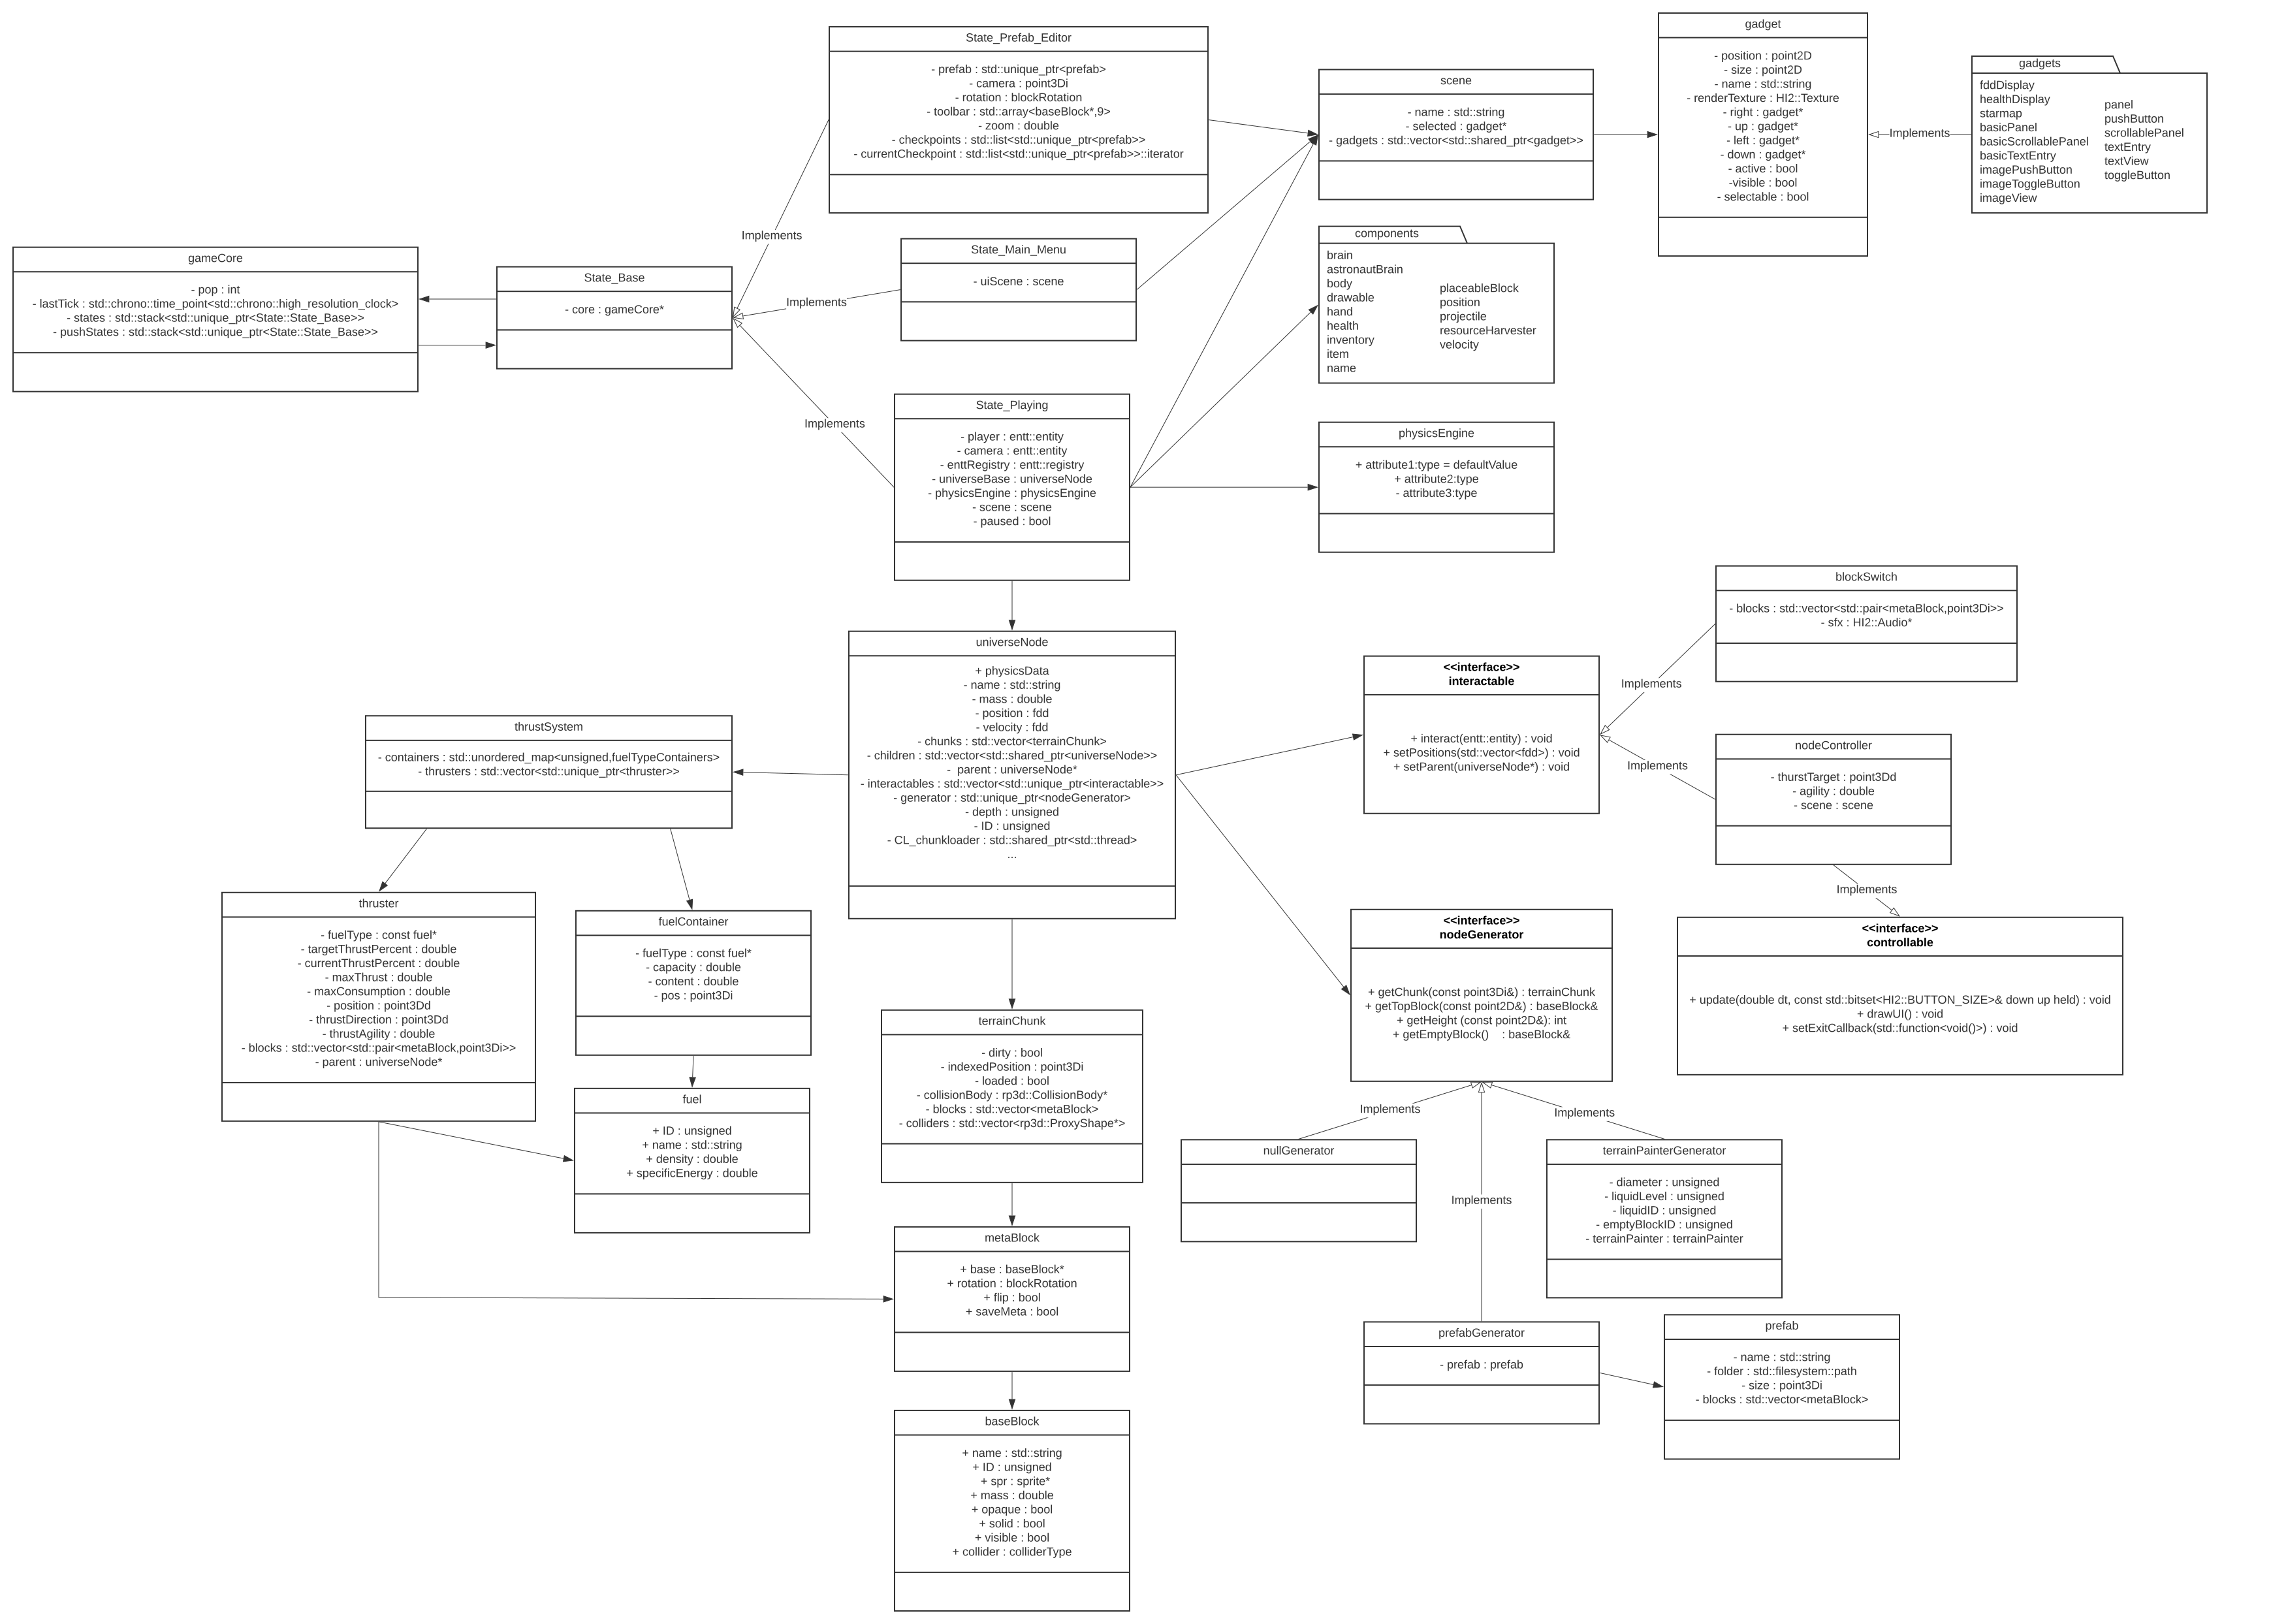
\includegraphics[angle=90,origin=c,scale=0.25]{ms4}
  \caption{Diagrama de classes general}
  \label{dc_general}
\end{figure}
\section{Interfície i menús}
%\begin{landscape}
  \begin{figure}[H]
    \centering
    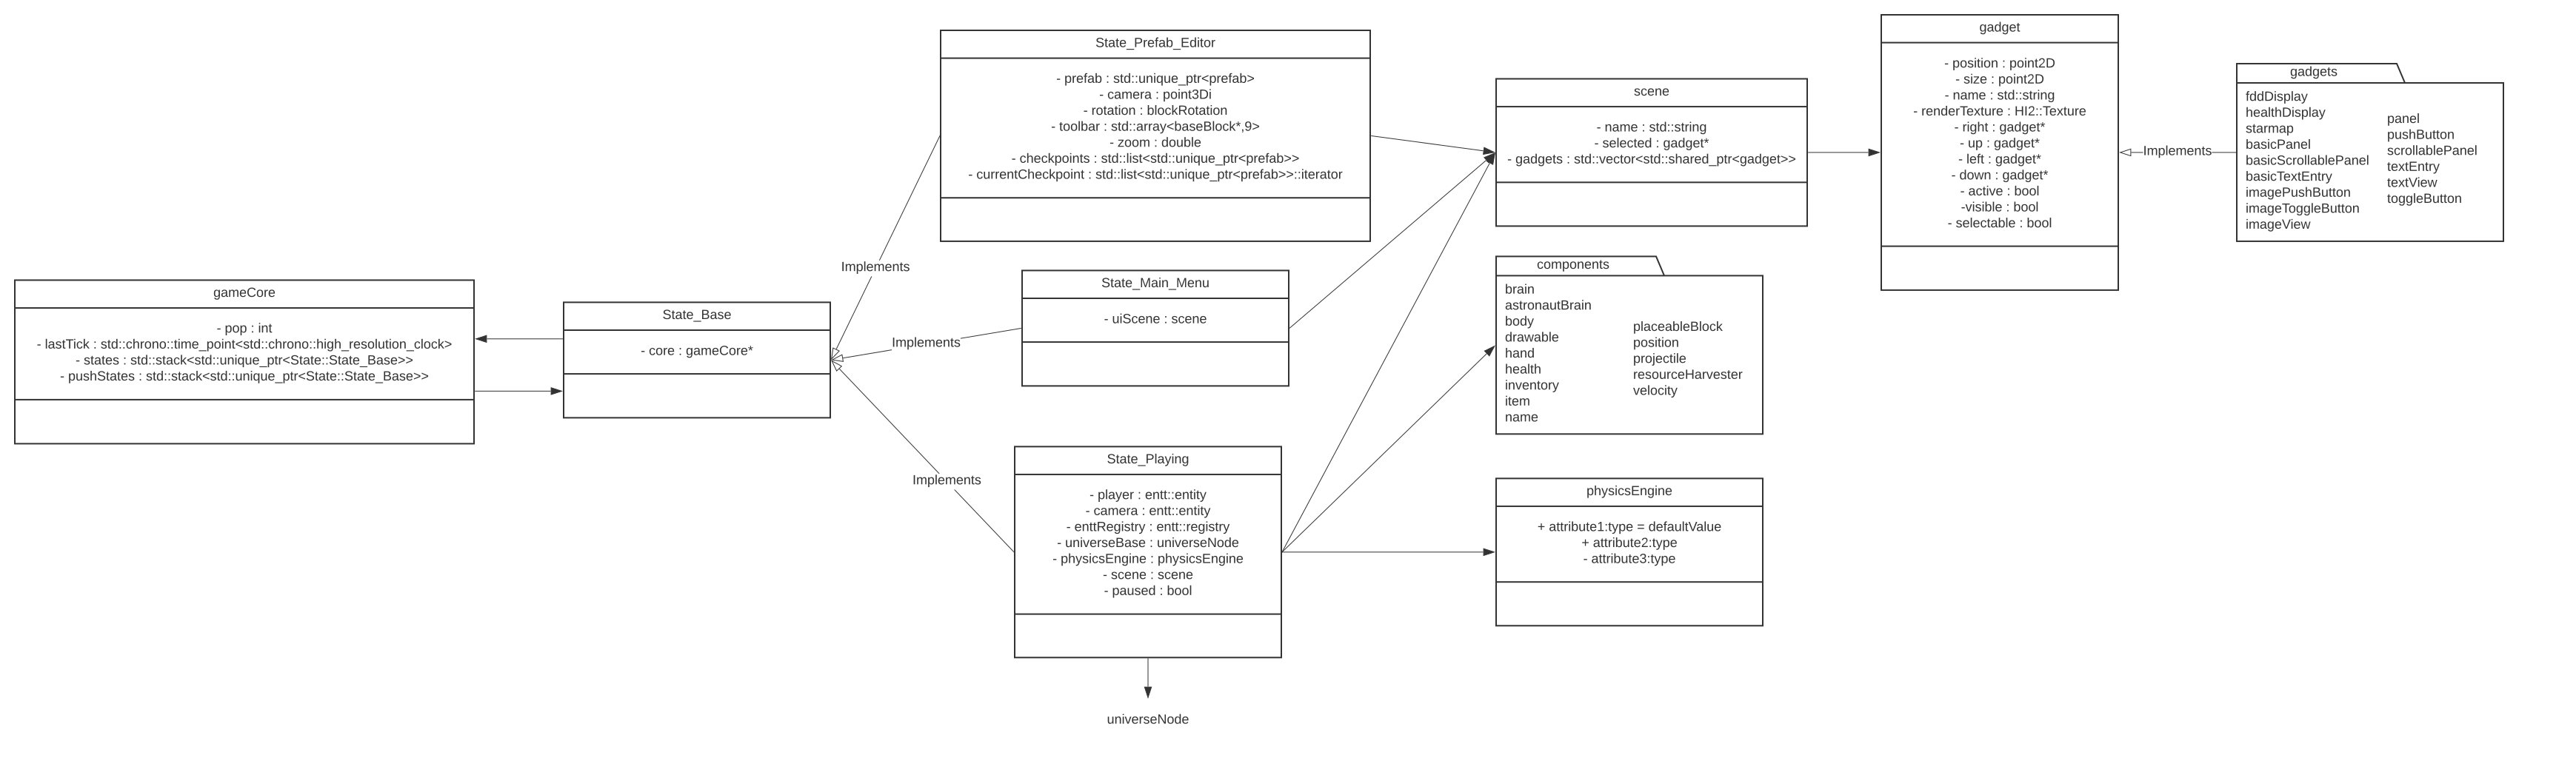
\includegraphics[angle=90,origin=c,scale=0.25]{ms1}
    \caption{Diagrama de classes de l'interfíce i menús}
    \label{dc_menu}
  \end{figure}
%\end{landscape}
En aquesta part es detallen les classes i el funcionament de la part menys relacionada amb el joc en sí. La separació és complicada de definir, però aqui s'explica el funcionament del bucle principal, els menús, el sistema d'estats i l'editor de `prefabs'. 
La funció `main' del nostre motor tant sols crea una instància d'un objecte gameCore, i acte següit crida la funció gameCore.gameLoop(), així que podríem considerar gameCore.gameLoop() com la nostre funció principal.
\subsection{gameCore}
%[[TODO-CLASSDIAG]]
La classe gameCore és l'encarregada de gestionar els diferents estats del motor. 
Simplement conté una pila d'estats, i la conté una funció que fa de bucle principal, la qual s'encarrega de cridar les funcions de \textit{input}, càlcul i dibuix del estat que estigui al cim de la pila.
Els pròpis estats podràn, aleshores, cridar funcions de gameCore per treure o afegir estats a la pila.

\subsection{States}
Els estats, o més concretament, State\_Base, és una classe abstracte que representa una escena o estat del motor. Conté mètodes per rebre \textit{input}, actualitzar l'estat i dibuixar-lo.
Exemples d'estats possibles podrien ser l'estat del menú principal, un estat per modificar les opcions del joc, l'estat de \textit{gameplay} en sí, o un estat de pausa dins del \textit{gameplay}.
A part dels estats que explicarem a continuació, hi ha l'estat del joc (State\_Playing) que serà explicat al apartat de simulació del joc.

\subsubsection{Main Menu}
Main\_Menu és l'estat que representa el menú principal. Conté molt poca lògica, ja que simplement és interfície gràfica per entrar a altres estats del motor.
\begin{figure}[H]
  \centering
  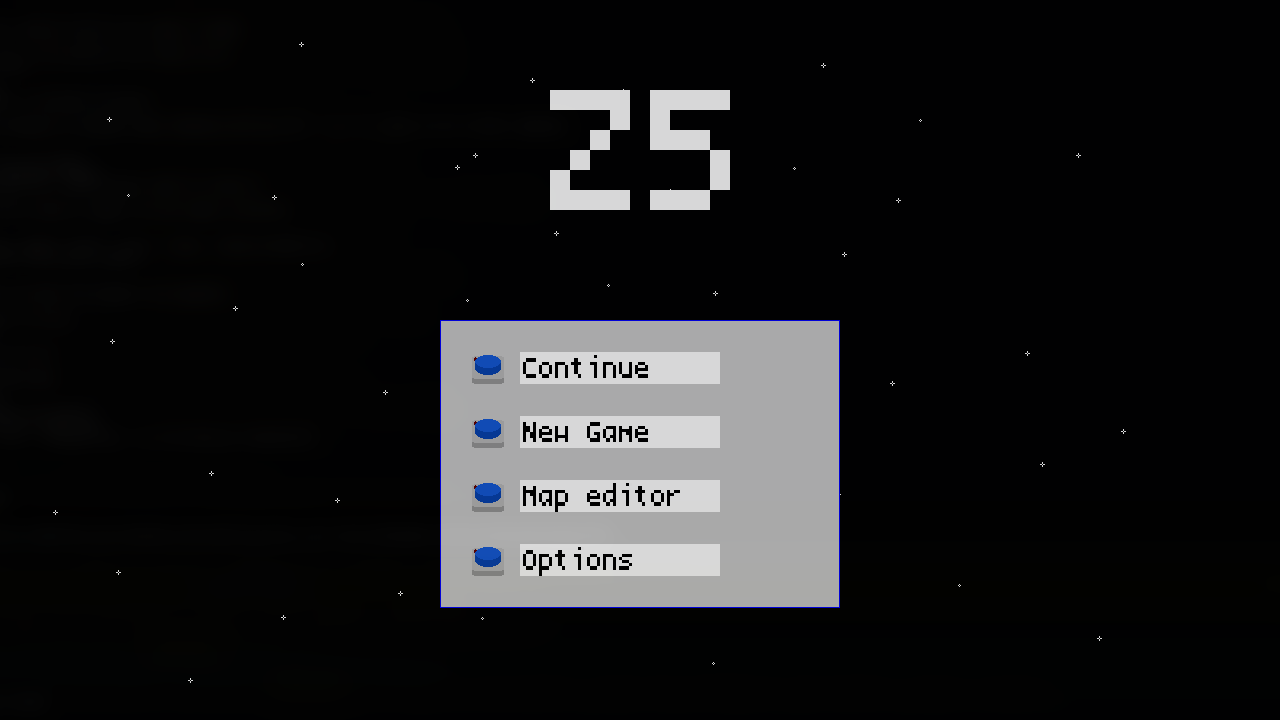
\includegraphics[scale=0.25]{menu}
  \caption{Captura de pantalla del menú principal.}
\end{figure}
\subsubsection{Prefab Editor}
Prefab\_Editor és l'estat del editor de prefabs del motor. Té un funcionament similar a una èina de dibuix informàtica, on l'usuari pot omplir una graella de píxels amb diferents colors, en aquest cas blocs, arrossegant el cursor per la pantalla.
Disposa d'eines de pinzell, esborrador, cub de pintura i seleccions. També incorpora funcionalitat per copiar, retallar, enganxar, desfer i refer canvis.
\\
Inclou una petita interfície d'usuari per sobre el llenç de dibuix, on es mostren els blocs que tenim disponibles per decorar el prefab. Tot i així, manca molt de feedback visual, ja que la majoria d'interaccions s'expressen a través de la consola mitjançant text, i les eines es seleccionen utilitzant draçeres de teclat.
\begin{figure}[H]
  \centering
  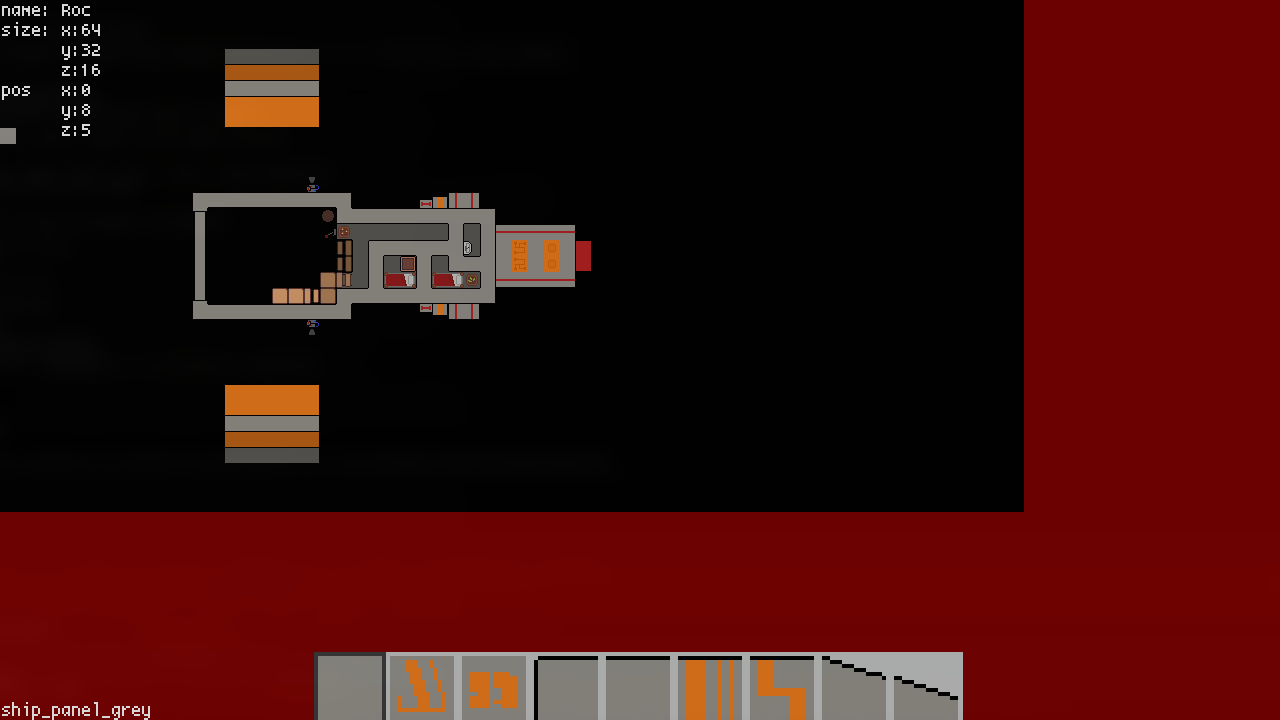
\includegraphics[scale=0.25]{prefabEditor}
  \caption{Captura de pantalla del editor de prefabs.}
\end{figure}

\subsection{UI}
Per l'interfície d'usuari s'ha implementat un petit framework fet des de zero prou senzill, amb l'objectiu de permetre al usuari interactuar tant amb teclat i ratolí com amb controls o comandaments de consola.
\\
La interfície d'usuari únicament disposa de dos components diferenciats.

\subsubsection{gadget}
%[[TODO-IMATGES]]
Un gadget és una classe abstracte que representa un element qualsevol de l'interfície d'usuari. Els gadgets s'encarreguen de gestionar la seva posició i tamany, la visibilitat, el nom, i mantenen enllaços als gadgets que tenen al voltant per poder-hi accedir direccionalment.
Els gadgets que hi ha actualment al motor són:
\begin{itemize}
  \item{panel: Gadget que representa un panell rectangular on es poden afegir altres gadgets.}
  \item{pushButton: Gadget que representa un polsador, amb el qual es poden prendre accions al ser premut.}
  \item{textView: Gadget que representa una caixa de text fixa.}
  \item{textEntry: Gadget que representa una caixa d'entrada de text.}
  \item{toggleButton: Gadget que representa un interruptor.}
  \item{imageView: Gadget que permet mostrar una imatge en pantalla.}
  \item{scrollablePanel: Gadget que especialitza un panell, i afegeix funcionalitat per un panell on existeix un `tamany intern' major al tamany del panell, amb el qual s'afegeix l'habilitat de desplaçar-nos per dins del panell.}
  \item{basicPanel: Gadget que especialitza un panell, i afegeix un fons sòlid al panell original.}
  \item{basicScrollablePanel: Gadget que especialitza un scrollablePanel, i afegeix un fons sòlid al gadget original.}
  \item{basicTextEntry: Gadget que especialitza un textEntry, i afegeix un fons sòlid al gadget original.}
  \item{imagePushButton: Gadget que especialitza un pushButton, i afegeix suport per que el gadget es mostri com a una imatge, amb la possibilitat de canviar d'imatge al mantenir-se apretat.}
  \item{imageToggleButton: Gadget que especialitza un toggleButton, i afegeix suport per que el gadget es mostri com a una imatge, canviant d'imatge segons l'estat del interruptor.}
  \item{fddDisplay: Gadget que representa un fdd de forma gràfica. Principalment utilitzat per propòsits de desenvolupament.}
  \item{healthDisplay: Gadget que permet mostrar per pantalla la salut d'una entitat.}
  \item{starmap: Gadget que mostra un mapa galàctic al voltant d'un cos astronòmic. Permet visualitzar les òrbites previstes d'un cos i les seves propietats (nom, massa i diàmetre)}
\end{itemize}
\begin{figure}[H]
  \centering
  \includegraphics[scale=5]{botons}
  \caption{Botons i interruptors de la interfície en estats actiu i inactiu.}
\end{figure}
\begin{figure}[H]
  \centering
  \includegraphics[scale=0.5]{starmap}
  \caption{Captura d'un starmap mostrant l'òrbita de Mart.}
\end{figure}
\begin{figure}[H]
  \centering
  \includegraphics[scale=0.5]{healthDisplay}
  \caption{Captura d'un healthDisplay amb quatre cors plens de cinc màxims.}
\end{figure}
\begin{figure}[H]
  \centering
  \includegraphics[scale=0.5]{fddDisplay}
  \caption{Captura d'un fddDisplay representant un vector amb direcció +X +Y +Z.}
\end{figure}

\subsubsection{scene}
L'escena és poc més que un contenidor de gadgets, s'encarregarà de mantenir un gadget com a seleccionat, i fer les crides recursives per dibuixar i interactuar amb els gadgets que la composen.

\section{Simulació del joc}
En aquesta part es detalla el disseny de la part de gameplay i simulació del motor. A grans trets, podríem dir que la classe principal és State\_Playing, que serà l'encarregada de rebre entrada, simular, i mostrar per pantalla l'acció del joc.
\begin{figure}[H]
  \centering
  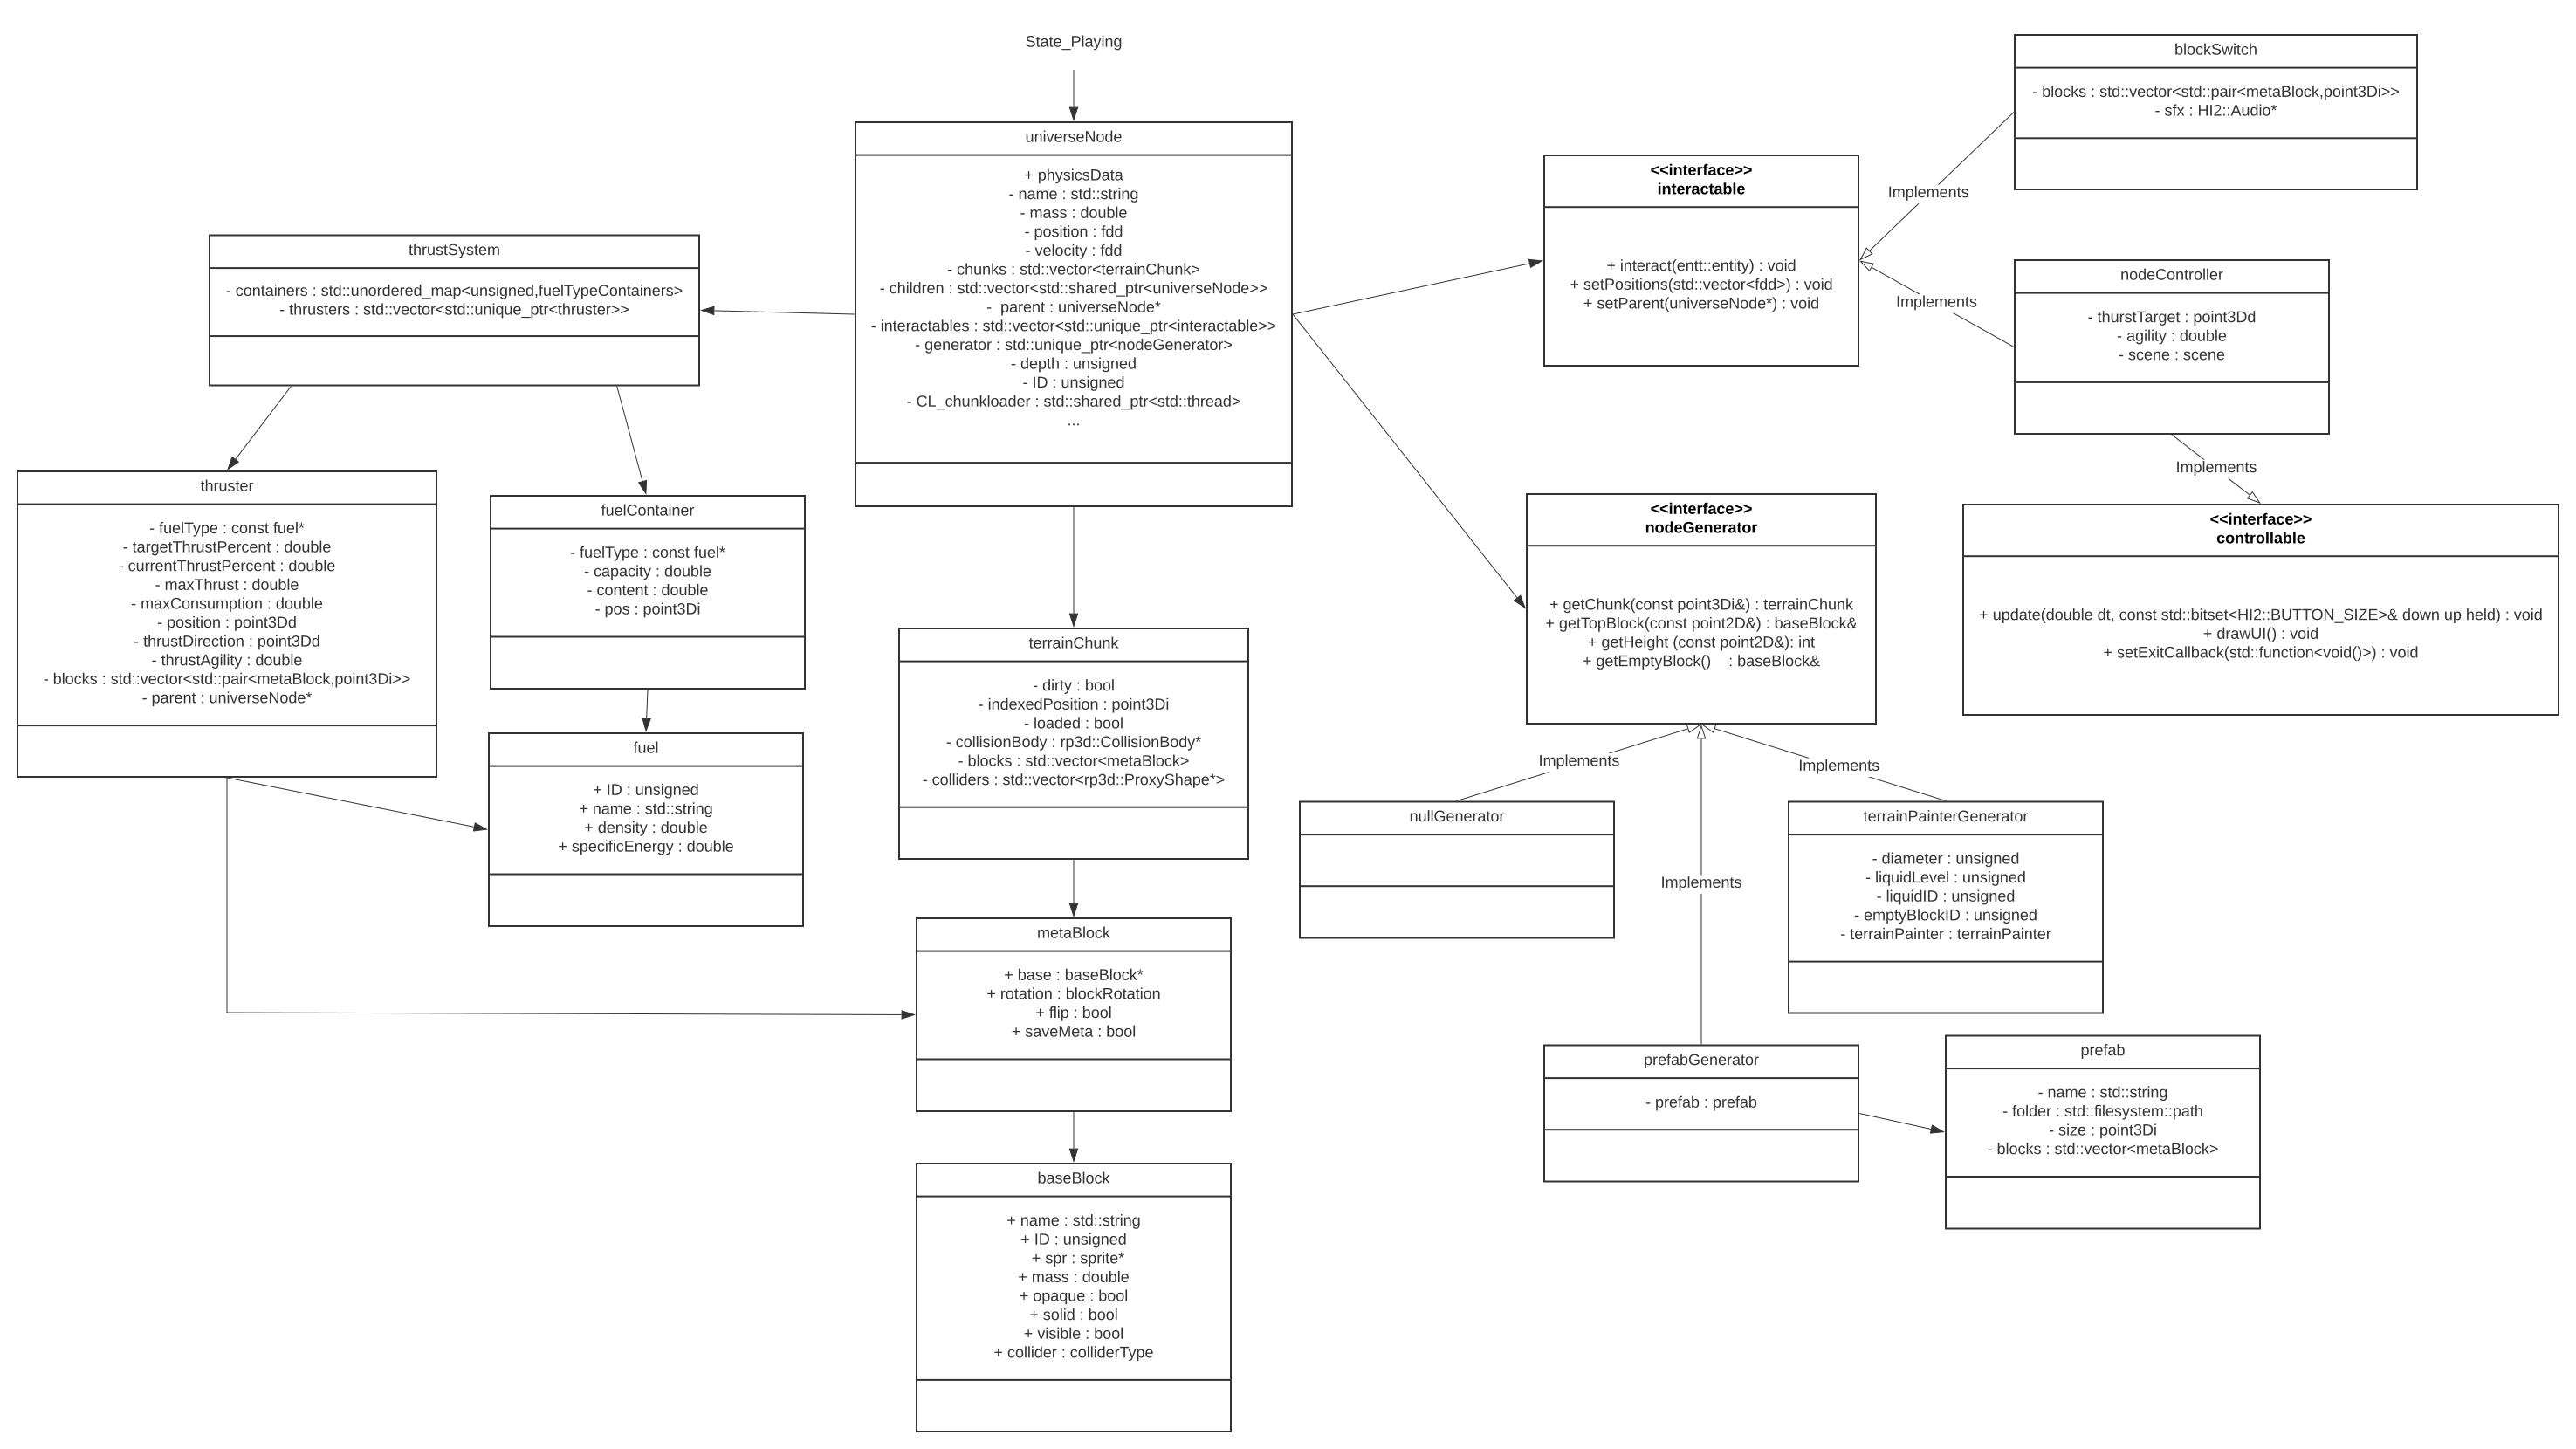
\includegraphics[angle=90,origin=c,scale=0.32]{ms2}
  \caption{Diagrama de classes de la part de simulació.}
\end{figure}

\subsection{Escena del joc State Playing}
%[[TODO-CLASSDIAG]]
State\_Playing és l'escena principal del joc, i és l'encarregada de gestionar els diferents sistemes de la simulació. Conté la `scene' de la UI, el registre d'entitats i el node base de la simulació. A continuació es detallen les seves funcionalitats més importants.
\subsubsection{Renderitzat}
Tot i que el nostre motor i simulació es realitzen en un espai tridimensional, el renderitzat es farà utilitzant sprites en 2D. 
Per tal de donar un efecte de profunditat, el procés de renderitzat consistirà en dibuixar els nodes capa a capa, aplicant parallatge a cada capa segons la seva distància amb la càmera. 
D'aquesta manera, les capes més profundes i llunyanes a la càmera es dibuixaran abans i amb un menor zoom, tal que al moure la càmera el moviment en píxels d'aquella capa serà menor i donarà l'efecte de ser més llunyana.
\\
Es podran renderitzar quatre tipus d'elements, nodes, entitats visibles, requadres i filtres de capa. Per gestionar les diferents profunditats es mantindrà una llista de capes a dibuixar, que seran posteriorment ordenades segons la seva profunditat. 
Els nodes es renderitzaran iterant per les capes del terreny i afegint-les a la llista. Tot node de la simulació serà considerat per renderitzar, però només ho serà en cas d'estar a una distància de la càmera que permeti que aparegui per pantalla. 
Seguidament s'afegiran a la llista totes les entitats dibuixables que es trobin en una alçada dibuixable per la càmera, i que estiguin a una distància raonable com per ser dibuixades.
S'afegiran multiples capes rectangulars translúcides, que donaràn un efecte de boira a les capes més llunyanes.
Finalment, s'afegirà un requadre al voltant del `interactable' més proper al jugador, en cas que n'hi hagi algun a l'abast.
\\
Tot seguit s'ordenaràn els elements a dibuixar afegits a la llista segons la seva profunditat respecte la càmera, en ordre de més llunyà a més proper.
Finalment començarà el procés de renderitzat pròpiament dit. Les capes de filtre tant sols necessitaran dibuixar un rectangle del seu color que cobreixi tota la pantalla. Entitats i requadre són simples de dibuixar, tant sols cal aplicar una transformació per convertir la seva posició relativa a la càmera en posició respecte l'orígen de la pantalla, i aplicar zoom segons la seva profunditat a l'hora de dibuixar.
\\
El renderitzat de capes de terreny serà lleugerament més complex. El procés consisteix en dibuixar els blocs de la capa un a un, iterant per aquells que es trobin dins el camp de visió de la càmera, aplicant efectes d'ombres i oclusió ambiental en cas de ser necessari.
Als blocs de les capes s'apliquen tres tècniques de pre/post-processat.
A cada bloc se li és calculada la seva visibilitat, a partir de la qual es decidirà si dibuixar o no el bloc. Aquesta visibilitat és precalculada al carregar el chunk que la conté. Es considera un bloc com a visible si qualsevol dels nou blocs situats en un quadrat de 3x3 centrat en el bloc de sobre del bloc actual és visible.
També es precalcula un efecte de oclusió ambiental, amb el que s'apliquen diferents ombres als blocs en funció dels blocs que té situats a sobre.
Finalment, a cada capa es calcula un ombrejat general segons la seva profunditat, donant tons més foscos a les capes més profundes i ajudant al jugador a entendre la profunditat de les capes.

\subsubsection{Entrada}
Per processar l'entrada simplement es passen les tecles i interaccions rebudes cap a l'escena de la UI, i s'envien també cap al component `brain' del jugador en cas que en tingui.
\subsubsection{Actualització}
En la fase d'actualització s'executen els sistemes del sistema entitat component, s'actualitzen els propulsors dels nodes, es netejen i s'adormen/desperten les entitats que escaiguin, i finalment es fan els càlculs de física i s'actualitza la càmera per evitar co\lgem isions.
\subsection{universeNode}
%[[TODO-CLASSDIAG]]
La classe universeNode servirà per representar els cossos astronòmics en la simulació (els anomenats nodes). Els nodes tenen una estructura jeràrquica, on cada node conté els seus nodes fills, que són els nodes que l'estan orbitant.
Els nodes contenen el terreny del joc, que està compost per múltiples agrupacions de blocs anomenades chunks. 
Cada node conté una matriu 3D de chunks, on aquests seran carregats en temps real mitjançant un fil para\lgem el d'execució.
Els nodes mantenen informació sobre la seva massa, diàmetre, el node pare, la seva posició i velocitat respecte al seu pare, el seu sistema de propulsió, el seu generador i la llista de `interactables' que contenen.
\begin{figure}[H]
  \centering
  \includegraphics[scale=0.15]{hier}
  \caption{Exemple de jerarquía de universeNodes. Sagitari A* és el node arrel, i cada node conté els seus nodes inferiors. La Terra conté la Lluna i la nau grossa (Roc), i dins la nau grossa tenim la petita (Sparrow).}
\end{figure}
\subsubsection{Reparentització}
Per tal de recalcular la jerarquía dels nodes, els nodes tenen un mètode que els permet calcular el millor pare donada una posició i un pare actual. Aquest càlcul es fa mitjançant esferes d'influència, que són un concepte utilitzat en astrodinàmica per calcular el principal cos al que un cos astronòmic orbita. A part de les esferes d'influència, tenen prioritat els nodes en els quals la posició donada correspongui a un bloc no buit.
\subsubsection{chunkLoader}
%[[TODO-IMATGE]]
Els chunkLoaders són fils d'execució que cada node conté. S'encarreguen de carregar nous chunks al voltant del jugador per tal que el jugador pugui moure's pel terreny sense cap pantalla de càrrega.
El funcionament a alt nivell és el següent:
\begin{enumerate}
  \item Es llegeix la posició del jugador respecte al node, la qual és calculada des de fora el fil i transmesa a través d'una variable compartida.
  \item En cas que la posició del jugador no hagi canviat de chunk, el chunkLoader adorm el fil durant un temps.
  \item En cas que que sí, els chunks més llunyans al jugador seràn carregats, en cas de ser a disc es carregaran des de disc, en cas contrari seran generats pel nodeGenerator.
\end{enumerate}
Per determinar on posicionar un chunk dins la matriu de chunks s'obté la posició del chunk en el món, es divideix cada eix entre el tamany del costat dels chunks, i finalment s'obté la posició dins de la matriu aplicant el mòdul del tamany dels costats de la matriu 3D.
D'aquesta manera s'aconsegueix un efecte similar a un buffer circular en tres dimensions.

\subsection{terrainChunk}
%[[TODO-IMATGE]]
Els terrainChunks són agrupacions cúbiques de blocs. Actualment són cubs de vuit blocs per costat, resultant en 512 blocs per chunk, tot i que el tamany dels chunks és un senzill paràmetre fàcil de canviar.
Els blocs, més concretament metaBlocks, es guarden en un vector i s'accedeix als blocs com si estiguessin en una matriu tridimensional.
Els chunks poden ser serialitzats i deserialitzats cap a disc, i es poden crear utilitzant el nodeGenerator del node que els contingui.
\subsection{Blocs}
Els blocs seràn el material amb el que el terreny del joc estarà construït. Representen un bloc de un metre cúbic. Dins del motor es fan servir dues classes per representar els blocs.
\begin{figure}[H]
\centering
\includegraphics[scale=3]{blocs}
\caption{Blocs de terra, gespa aigua i sorra.}
\end{figure}

\subsubsection{baseBlock}
El struct baseBlock representa un bloc imaginari amb unes certes propietats. Les propietats inclouen nom, ID, visibilitat, si és sòlid, opacitat, massa, colisionador i sprite.

\subsubsection{metaBlock}
Els metaBlock en canvi representen un bloc real d'un node. Contenen una referència al baseBlock que representen, pero a més contenen informació sobre la rotació del bloc, visibilitat, i oclusió ambiental.
Els chunks de terreny estàn doncs formats per multiples metaBlocks, els quals fan referència a un baseBlock que no es pot modificar. Podríem considerar aquesta separació com a una aplicació del patró \textit{flyweight}, el qual ens permet evitar informació redundant de manera dràstica.
\subsection{Interactables}
Interactable és una classe abstracte per a blocs especials amb els que les entitats hagin de poder interactuar. Són un concepte similar a entitats, però amb la diferència que estan relacionades amb un o múltiples blocs, i estan emmagatzemades en els nodes enlloc de pertànyer a un registre global.
Un mateix interactable pot tenir múltiples posicions des de les quals pot ser accionat.
\subsection{nodeController}
%[[TODO-IMATGE]]
Els nodeController són un tipus de interactable que permeten a una entitat controlar el sistema de propulsió d'un node. Permeten a la entitat establir un objectiu de propulsió, i el sistema de propulsió serà dirigit per tal que el node es mogui cap aquell objectiu.
\subsection{blockSwitch}
%[[TODO-IMATGE]]
Els blockSwitch són un interactable que permet a una entitat canviar un grup de blocs per un altre. Aquest interactable serveix principalment per a fer portes i interruptors per a portals.
\subsection{Entitats i components}
Com ja s'ha introduït anteriorment, les entitats son part del patró entity component system que fem servir per modelar els actors i objectes del joc. En la majoria de casos son senzilles estructures que guarden informació, com per exemple la salut del personatge, però no estan limitades a només això.
\subsubsection{brain}
El brain és una classe abstracte que representa un component que controla una entitat. Aquest brain és actualitzat regularment pel sistema, i en cas de pertànyer al jugador s'actualitzarà a partir del botons i tecles que l'usuari hagi apretat.
En cas contrari, els brain poden implementar funcionalitat per actuar com a inteligència artificial per les entitats.
Actualment tant sols hi ha una classe que implementi brain, la qual explicarem en el següent punt.
\subsubsection{astronautBrain}
%[[TODO-FIGURA]]
El component astronautBrain és una classe que implementa brain. Conté una màquina d'estats que exposaràn diferent funcionalitat al jugador depenent de cada situació.
Per exemple, al estar en contacte amb el terra la entitat es considerarà "grounded", i tindrà accés a caminar i saltar. 
En saltar, el brain passarà a un estat on està saltant, i comença a incrementar la seva velocitat respecte l'eix vertical.
Tot seguit, al perdre contacte amb el terra el brain passarà a estat "airborne" o volant/flotant, i tindrà accés a uns petits propulsors que permetràn al usuari controlar el personatge lleugerament, en cas d'estar volant o flotant a l'espai.
Quan el personatge torni a estar en contacte amb el terra tornarà a estar al estat "grounded" i tornarà a tenir accés a les opcions d'aquell estat.
Aquesta màquina d'estats permet modelar comportaments prou complicats, on cada estat pot portar a diversos altres estats depenent de l'acció que s'hagi près.
Actualment aquest component no implementa cap inte\lgem igència artificial per a entitats que no siguin el jugador.
\subsubsection{body}
Body és una estructura que representa un cos físic esfèric. Conté informació sobre el seu diàmetre, massa, volum i elasticitat. Aquest cos aleshores serà utilitzat pel motor de física per calcular co\lgem isions i efectes similars.
\subsubsection{drawable}
Drawable és una estructura que representa un sprite dibuixable. Conté a dins una referència a un sprite, el nom del sprite i una variable zoom que permet ampliar o reduïr el tamany del sprite.
\subsubsection{hand}
Hand és una estructura que modela una mà com a recipient per a un objecte. Una mà pot estar agafant un objecte, i en cas de ser accionable, l'objecte podrà ser accionat.
\subsubsection{health}
Health és una classe que representa la salut de la entitat. La entitat que tingui component de health podrà ser danyada i curada, i en cas d'arribar a zero salut, la entitat serà esborrada del joc.
\subsubsection{inventory}
Inventory és una classe que modela un inventari, que és una co\lgem ecció d'objectes. Aquests objectes podràn fer-se servir a través de la mà, en cas que la entitat en tingui.
\subsubsection{item}
Item modela un objecte, o múltiples objectes del mateix tipus. Aquests objectes poden estar caiguts al terra, o bé estar al inventari d'una altre entitat.
\subsubsection{name}
Component que modela el nom d'una entitat. Actualment no té cap ús dins del joc, i només es fa servir en alguna comanda de \textit{debugging} per identificar entitats.
\subsubsection{placeableBlock}
Item interactuable que permet posicionar un bloc cap on la entitat que l'acciona està mirant.
\subsubsection{resourceHarvester}
Item interactuable que permet extreure blocs del terreny, convertint-los en items que les entitats poden recollir i co\lgem ocar.
\subsubsection{position}
Estructura que modela la posició d'una entitat. Al igual que amb els nodes, la posició és relativa a un node pare, i la posició en sí és del tipus fdd.
\subsubsection{projectile}
Component que modela un projectil que causa dany a les entitats amb que impacta. Emmagatzema informació sobre el dany del projectil, les vegades que encara pot rebotar en el terreny, els enemics que encara pot atravessar, i la ultiam entitat amb qui ha impactat, per tal de no registrar multiples impactes en la mateixa entitat.
\subsubsection{velocity}
Component que modela la velocitat de la entitat. Tot i que és relativa al node pare, no emmagatzema cap referència al pare, ja que ja hi és en el component posició.
\subsection{thrustSystem}
%[[TODO-CLASSDIAG]]
El thrustSystem és una classe encarregada de modelar tot el sistema de propulsió d'un node. Gestiona els propulsors i contenidors de combustible del node.
S'ocupa de gestionar la consumpció i recàrrega de combustible, tinguent en compte els diversos tipus de combustible i els contenidors corresponents a cada tipus. També s'encarrega d'alimentar els propulsors i gestionar la seva potència per tal de dirigir el node cap al objectiu.
\subsubsection{fuel}
El fuel és una senzilla estructura que representa un tipus de combustible. Conté un identificador, un nom, la densitat en $kg/m³$ i la energía específica en $MJ/kg$.
\subsubsection{fuelContainer}
Un fuelContainer representa un contenidor d'un cert tipus de combustible. Manté la seva capacitat màxima, el contingut actual, el tipus de combustible que admet i la posició on es troba.
\subsubsection{thruster}
Un thruster modela un propulsor d'un cert tipus de combustible. Emmagatzema informació sobre el tipus de combustible que admet, el seu objectiu de potència, la seva potència actual, la propulsió que ofereix al estar a màxima potència, i la quantitat de combustible que consumeix a màxima potència, a més de la seva posició, agilitat i orientació.
El seu canvi de potència no és instantàni, sinó que es modela a partir de la potència actual i la agilitat del propulsor. D'aquesta manera, al intentar encendre els propulsors a màxima potència aquests han de augmentàr de potència fins arribar a la màxima.
\subsection{prefab}
%[[TODO_IMATGE]]
La classe prefab representa un conjunt de blocs prefabricat. És creat amb l'editor de prefabs, i després utilitzat pels nodes que utilitzin un prefabGenerator. Conté el seu nom, les seves dimensions i el vector de metaBlocks que el composen.
\subsection{nodeGenerator}
%[[TODO-CLASSDIAG]]
NodeGenerator és una classe abstracte que serveix per representar un generador de node. Aquest generador serà cridat pel node quan aquest necessiti carregar un chunk que no hagi trobat a disc. En aquest cas el nodeGenerator fabricarà un chunk i li donarà al node. També ofereix mètodes per obtenir el bloc de la superfície en un punt concret, l'alçada del terreny en un punt, o per saber quin és el bloc que s'utilitza per l'espai buit en aquell node.
Actualment hi ha tres tipus de generadors implementats, que es detallen a continuació.
\subsubsection{nullGenerator}
NullGenerator és un nodeGenerator \textit{stub}, que serveix principalment per a propòsits de \textit{debugging} o per aquells nodes que siguin construïts per un jugador.
\subsubsection{prefabGenerator}
PrefabGenerator és un nodeGenerator que genera chunks a partir d'un prefabricat. Això ens serveix per generar estructures fetes a mà com per exemple naus, estacions espacials, ciutats, asteroides o qualsevol altre tipus de node que un dissenyador pugui crear a mà.
Tot i qué té gran utilitat per crear estructures estàtiques, no és capaç de generar estructures amb portes o blocs interaccionables, ja que aquests no es troben a nivell de chunk sinó a nivell de node.
\subsubsection{terrainPainterGenerator}
TerrainPainterGenerator és el principal generador per a terreny del motor. Genera cossos astronòmics a escala real però de forma cilíndrica.
Funciona a partir de fer un mostreig al gradient de soroll a partir de la posició 2D del bloc a calcular. Un cop es té el nivell de soroll en aquell punt, s'utilitza una llista de seccions de terreny a les quals el soroll està mapejat, per tal d'obtenir el bloc que tocarà a aquella alçada tinguent en compte el soroll de la posició 2D.
\begin{figure}[H]
  \centering
  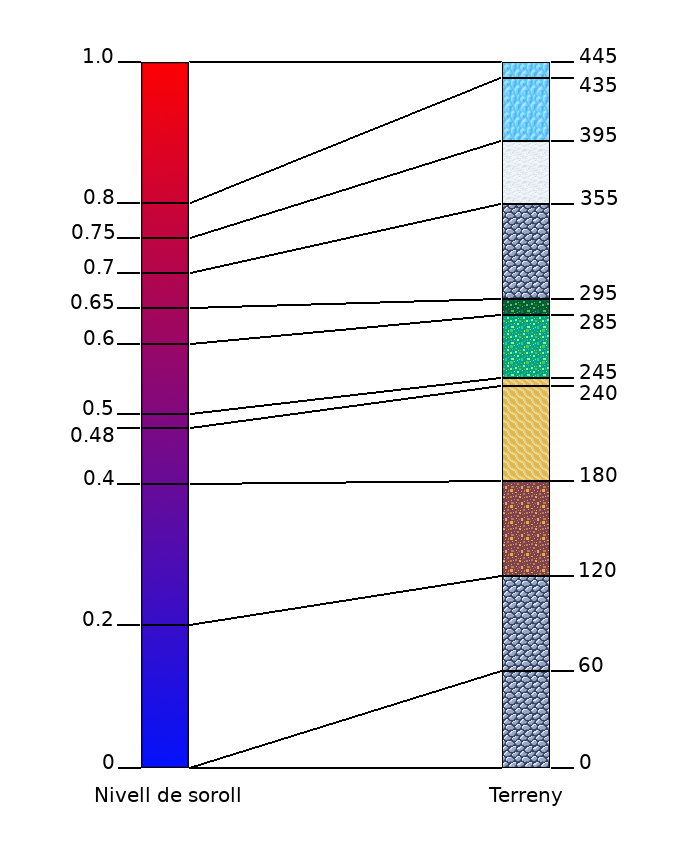
\includegraphics[scale=1.5]{mappingGradient}
  \caption{Representació del mapeig entre soroll i terreny al planeta Gaia.}
\end{figure}

\subsection{physicsEngine}
PhysicsEngine és la classe que representa el motor de física, i és la encarregada de fer tots els càlculs de física del motor. És filla de la classe rp3d::CollisionCallback degut a necessitats per utilitzar la llibreria de física. 
En totes les co\lgem isions s'aplicarà un petit factor de pèrdua d'energia per simular l'energia convertida en calor, i així evitar sistemes de moviment perpetu.
\subsubsection{Gravetat}
El càlcul de gravetat s'aplica a tot node i entitat de la simulació.
La lògica és la següent:
Si el node té gravetat artificial, es torna directament com a acceleració resultant la establerta segons la gravetat artifical.
En cas contrari, es calculen dues gravetats, la "màgica" i la real. La real és la gravetat normal calculada utilitzant la fòrmula de la gravitació universal de Newton $F=G\frac{m_{1}m_{2}}{r²}$. A partir de la força i la massa del objecte obtenim una acceleració utilitzant $F=ma$.
També és calculada la gravetat "màgica", que és la equivalent a la gravetat real a la superfície del planeta en cas que aquest fós esfèric. La màgica, però, sempre és en direcció cap a la Z negativa, per tal que els planetes cilíndrics no arrastrin els cossos cap al centre, sinó que els atreguin cap al terra (-Z).
Tot següit es calcula un factor de "màgia", que decidira quin percentatge de gravetat màgica i quin de real s'aplica al cos.
Aquest factor és sempre 1 mentre el cos estigui en la superfície del node, però ràpidament decau cap a 0 linealment al sortir del perímetre del cos. D'aquesta manera obtenim una gravetat que va cap a -Z al estar a sobre la superfície del planeta o cos, però tenim gravetat real que va cap al centre de massa del cos al sortir de la superfície d'aquest, habilitant la possibilitat d'orbitar qualsevol cos amb suficient massa.
\subsubsection{Propulsors}
Per calcular l'efecte dels propulsors en els nodes simplement hem de sumar l'efecte de tots els propulsors. Per obtenir l'efecte de cada propulsor hem de multiplicar la seva potència màxima en Newtons pel percentatge de potència actual. Amb aquesta força podem aplicar $F=ma$ per obtenir la acceleració resultant.
\subsubsection{Flotabilitat}
Per calcular la flotabilitat de cossos i entitats fem servir la fòrmula $F_{b}=\rho fVg$, on $Fb$ és la força resultant, $\rho f$ és la densitat del fluid, $V$ és el volum de fluid desplaçat i $g$ és la acceleració gravitacional del cos submergit. Per les entitats podem trobar el volum a través de les dimensions del seu body. Per els nodes aproximem el volum utilitzant el seu diàmetre i assumint que té forma d'esfera.  Pot semblar una aproximació poc refinada, però els resultats que dóna son suficientment bons. Tot i que va ser esborrada, la flotabilitat va permetre afegir una funció amb la que els personatges podien controlar la seva flotabilitat dins l'aigua a través d'aguantar la respiració, i per tant augmentar o disminuïr el seu volum. 
\subsubsection{Fricció aerodinàmica}
Pels càlculs de fricció aerodinàmica fem servir la fòrmula $F=0.5\rho u²C_{p}A$, on $F$ és la força resultant, $\rho$ és la densitat del fluid, $u$ és la velocitat del flux respecte l'objecte, $A$ és l'àrea on s'aplica la fricció, i $C_{p}$ és el coefficient de fricció. La velocitat del plux s'assumeix com a igual a la velocitat del objecte submergit, l'àrea és calculada com la meitat d'una esfera, i el coefficient de fricció utilitzat és 0.25, que aproxima un cos suficientment aerodinàmic.
\subsubsection{Velocitat}
Amb les noves velocitats calculades només resta calcular les noves posicions de nodes i entitats a partir de la velocitat del cos i el temps transcorregut. A part d'aplicar aquesta velocitat per trobar la nova posició, de forma desacoblada al motor de física es calculen posicions extrapolades que permeten mostrar moviments suaus en pantalla tot i que la taxa d'actualització de posicions sigui de tant sols 20Hz.
\subsubsection{Co\lgem isió entre nodes}
Per calcular i resoldre les co\lgem isions entre nodes el que farem serà iterar per tots els nodes. A cada node comprovarem si és possible que co\lgem isioni amb el seu node pare, o amb els seus nodes germans, revisant si les seves AABBs es superposen, i en cas afirmatiu comprovarem les co\lgem isions dels chunks carregats dels nodes.
En cas que s'hagi produït una co\lgem isió, resoldrem les posicions i velocitats a partir de la normal del contacte, la velocitat del objecte petit i la profunditat del contacte. Mourem cap enrere el cos petit en direcció contrària a la seva velocitat fins que estigui just tocant el segon cos, aleshores calcularem la direcció de la nova velocitat reflectint la antiga respecte la normal del contacte. Finalment compensarem el moviment que hem retrocedit aplicant-lo de nou amb la nova velocitat.
No farem cap tipus de modificacions en l'objecte gran, ja que en la majoria de casos l'efecte seria negligible, i podria causar problemes al no simular la gravetat dels cossos fills respecte al pare, ja que un cos petit a la superfície d'un cos amb suficient gravetat acabaria accelerant al propi cos que genera la gravetat cap a la direcció d'aquesta.
En una estructura de nodes plana, aquesta fase és $\mathcal{O}(\frac{n²}{2})$ ja que comprovariem tots els nodes entre sí, però no repetiriem les comprovacions simètriques.
\subsubsection{Co\lgem isió entre entitats}
En les entitats seguirem un procés similar al dels nodes, però farem la simulació completa d'un xoc elàstic. Això vol dir que es recalcularan les posicions i velocitats de les dues entitats que hi intervinguin.
Comprovarem co\lgem isions entre entitats properes, i com amb els nodes, evitarem comprovar dues vegades la mateixa co\lgem isió revisant que l'identificador de la primera entitat sigui més gran que la de la segona.
Aquesta fase també és $\mathcal{O}(\frac{n²}{2})$.
\subsubsection{Co\lgem isió entre entitat i node}
Per les co\lgem isions entre entitats i nodes comprovarem la co\lgem isió amb el node pare de la entitat, i tots els fills d'aquest. En cas de que les AABB es superposin aleshores es farà la comprovació més detallada respecte als chunks de terreny. Només modificarem posició i velocitat de la entitat, ja que gairebé sempre tindrà una massa extremadament inferior a la del node.

\section{Utilitats}
En aquest apartat analitzarem certes classes i utilitats senzilles que no poden existir de forma individual, o que es fan servir en tot el motor, i per tant, no són classificables com a \textit{gameplay} o interfície.

\subsection{fdd}
Els fdd són una estructura que representen una posició tridimensional amb una rotació. Utilitzen nombres de coma flotant per representar amb gran precisió les posicions, però també oferint flexibilitat per a grans distàncies.
Contenen mètodes per convertir-los a punts 2D, 3D, per importar des de rp3d::Vector3, punts 3D, i diverses funcions per a operacions, com per exmeple el producte escalar, producte vectorial, càlculs d'angles i magnituds, entre d'altres.
\subsection{services}
En el projecte hi ha diversos sistemes als que cal tenir accés des de molts punts del motor. Per tal de no contaminar l'espai de noms global amb variables estàtiques, hi ha certs objectes que posarem a disposició del motor a través de variables estàtiques dins d'un espai de noms anomenat "services".
Services conté gestors de audio, gràfics, fonts i co\lgem isionadors, així com el registre d'entitats i el gestor de memòria de la física.
\subsection{config}
També tenim un espai de noms anomenat "config" on tenim diversos paràmetres configurables del motor. Alguns d'ells es poden configurar en temps d'execució, mentre d'altres són constexpr per necessitats de la implementació, o per facilitar optimitzacions al compilador.
Els paràmetres ajustables són:
\begin{itemize}
  \item El tamany del contenidor de chunks que té cada node (chunksContainerSize).
  \item Un paràmetre per activar o desactivar el renderitzat (render).
  \item El tamany de l'esfera al voltant de la càmera en la qual el chunkLoader carrega nous chunks (chunkloadSphereRadius).
  \item El nombre de blocs per costat de cada chunk (chunkSize).
  \item La profunditat màxima en que el renderitzat pot dibuixar una capa (cameraDepth).
  \item El tamany dels costats dels sprites (spriteSize).
  \item El zoom de la càmera (zoom).
  \item Dos paràmetres que permeten ajustar la profunditat de camp de la càmera (depthScale i minScale).
  \item L'alçada a la que la càmera es mantindrà sobre el jugador (cameraHeight).
  \item Un multiplicador de la velocitat de les òrbites (orbitDebugMultiplier).
  \item La distància en que una entitat pot interactuar amb un interactable (interactableRadius).
  \item La distància respecte la càmera amb la que les entitats no permanents seràn destruïdes (destroyDistance).
  \item El freqüència del motor de física (physicsHz).
  \item El nombre de passes del solucionador de co\lgem isions entre nodes i entitats (physicsSolverIterations).
  \item Un paràmetre per activar i desactivar el renderitzat d'ombres segons profunditat de la capa (drawDepthShadows).
  \item Un paràmetre per activar la extrapolació de posicions per al renderitzat (extrapolateRenderPositions).
  \item Un paràmetre per ajustar la profunditat en que s'activen les ombres (minShadow).
  \item Un paràmetre per activar i desactivar la gravetat (gravityEnabled).
  \item Un paràmetre per activar i desactivar la fricció (dragEnabled).
  \item Un paràmetre per activar i desactivar la oclusió ambiental (AOEnabled).
  \item La extensió dels sprites que fem servir (spriteExtension).
  \item La extensió del audio que fem servir (audioExtension).
  \item La extensió de les fonts que fem servir (fontExtension).
  \item El nombre de vegades que es pot fer Ctrl+Z al editor de prefabs (pfbEditorMaxCheckpoints).
\end{itemize}

\subsection{Sprites}
Els sprites són una classe que representa un sprite animat. Estàn associats a una sola textura, però contenen un vector de quadres que especifiquen diverses regions de la textura. Gestiona una referència al quadre actual, i avançant regularment de quadre dona l'efecte d'animacions.
\subsection{Gestors de recursos}
Les classes audioManager, fontManager, graphicsManager i colliderManager són classes que s'encarreguen de gestionar la creació, accés i destrucció de recursos que es fan servir en la aplicació. Ofereixen funcions per obtenir un recurs a partir del seu nom, i el gestor de forma transparent l'oferirà, carregant-lo de disc si cal.
Són tots molt similars, amb la diferència que el de gràfics gestiona Textures i Sprites, i el de co\lgem isionadors té un funcionament lleugerament diferent degut que ha de gestionar els recursos amb rp3d::.
\subsection{Observer}
L'Observer és una classe que proporciona un sistema d'esdeveniments al motor. Permet definir events associats a un tipus de dades, que podran ser llençats des de qualsevol part del motor. Un cop enviat l'esdeveniment, les dades seràn entregades als subscriptors d'aquell tipus d'esdeveniment.

\section{Llibreries}
A continuació es detalla el funcionament de les llibreries que fem servir pel projecte.
\subsection{HardwareInterface}
HardwareInterface és la llibreria que hem creat al llarg del desenvolupament del projecte per separar el codi dependent de cada plataforma en una capa separada.
Ofereix classes per representar textures, àudio, fonts i colors, a més de les estructures per representar punts en 2D i 3D. Ofereix una interfície per dibuixar píxels, rectangles, text i textures, per reproduïr audio, inicialitzar i tancar netament el sistema, i interactuar amb les tecles i joysticks entre d'altres funcions.
Si bé les implementacions de Switch i PC estan ambdues fetes amb SDL2, fent que siguin prou similars, hi ha funcions que sí difereixen, com per exemple la d'obtenció de input, o la inicialització i neteja del sistema, que a consola requereix encendre diversos serveis i apagar-los manualment.
\subsubsection{SDL2}
SDL2 és fet servir dins de HardwareInterface per implementar la gestió de finestres, audio, gràfics i entrada. La interfície que ofereix la llibreria és C, així que molta de la interacció amb SDL2 es fà a través de punters, castings, i gestió manual de memòria.
\subsection{EnTT}
EnTT ens presenta dos tipus de dades principals, el registre i les entitats. Les entitats són simplement un identificador per a agrupacions de components del registre. El registre, en canvi, és una classe més completa que farà tota la gestió dels components i entitats del sistema. Ens permet crear i destruïr entitats, afegir i treure components a les entitats, obtenir "vistes" del registre segons filtres de cerca, i manipular els components de les "vistes" obtingudes.
\subsection{ReactPhysics3D}
ReactPhysics3D ens ofereix totes les utilitats relacionades amb els càlculs de física del motor. Principalment ens permet crear cossos, que són agrupacions de simples polígons, els quals podràn co\lgem ionar amb altres cossos. Les co\lgem isions es comproven manualment entre cossos, i en cas que hi hagi un contacte ens serà informat, obtinguent dades sobre la normal del contacte, la profunditat i els cossos involucrats. 
Tot i ser una llibreria de C++, la gestió de memòria és manual, i requereix construïr i destruïr manualment els objectes de la llibreria.
\subsection{nlohmann/json}
Nlohmann/json ens ofereix una senzilla interfície per crear i parsejar arxius JSON\@. Cada classe a serialitzar ha de implementar les funcions to\_json() i from\_json, que s'encarregaràn de serialitzar i deserialitzar des d'arxius.
Totes les classes de la simulació excepte el terrainChunk i el prefab són serialitzables a JSON, i aquestes dues que no ho són implementen la serialització directament.
\subsection{FastNoise}
FastNoise ens ofereix la classe FastNoise, que és un generador de soroll generalitzat amb el que podem cridar les diferents funcions de soroll. Ens permet canviar freqüència, tipus de soroll, els paràmetres del fractal i la llavor del soroll entre d'altres.
\subsection{IceCream-Cpp}
IceCream-Cpp presenta la macro IC(), que facilita el "print debugging", admetent múltiples paràmetres de tipus variats, i presentant-los per consola de forma entenedora.

